\documentclass[]{article}

\usepackage[paperheight=18cm,paperwidth=14cm,textwidth=12cm]{geometry}
\usepackage[skip=20pt plus1pt, indent=40pt]{parskip}

\usepackage{hyperref}

\usepackage{graphicx}
\graphicspath{ {./images/} }
\usepackage{float}

\usepackage{amsmath}
\usepackage{amsfonts}
\usepackage{amssymb}

\usepackage{xcolor}
\usepackage{sectsty}
\definecolor{bittersweet}{rgb}{1.0, 0.44, 0.37}
\definecolor{grey}{rgb}{0.25, 0.25, 0.28}
\definecolor{black}{rgb}{0, 0, 0}
\subsubsectionfont{\color{black}}
\subsubsectionfont{\color{grey}}
\sectionfont{\color{bittersweet}}

\usepackage[T1]{fontenc}
\renewcommand\familydefault{\sfdefault} 

\usepackage{bm}

\newcommand{\ev}{\mathbb{E}[X]}
\renewcommand{\ev}[1]{\mathbb{E}[#1]}
\newcommand*{\diff}{\mathop{}\!\mathrm{d}}

\newcommand{\definizione}{\paragraph{Definizione:}}
\newcommand{\formula}{\paragraph{Formula generica:}}

\newcommand{\highlight}[1]{\colorbox{yellow}{$\displaystyle #1$}}

\begin{document}
    \tableofcontents
    \newpage 
    \section{Introduzione}
    In probabilità quello che facciamo noi è quello di supporre che le nostre distribuzioni siano \textbf{note}. \\
    in statistica facciamo il contrario, ossia dire qualcosa (anche detto \textit{fare dell'inferenza}) su \textbf{parametri sconosciuti}. \\
    Dato che i parametri sono scimage.pngonosciuti il massimo che possiamo fare è quello di ottenere \textit{una stima} dei parametri \textit{incogniti}. \\[2ex]
    Codesti signorini sono chiamati \textbf{stimatori puntuali} e sono indicati con il simbolo $\boldsymbol{\hat{\theta}}$ (in questo caso stiamo parlando di uno stimatore del parametro incognito $\boldsymbol{\theta}$) \\[2ex]
    Esisono anche gli \textit{stimatori non puntuali}, noti come \textbf{intervalli di confidenza}, ossia un intervallo di valori in cui può essere contenuto il \textit{dato incognito}.
    \paragraph{Esempio} $\hat{\theta}? \quad \text{Altezza della popolazione}$ \\[2ex]
    \begin{minipage}{0.49\textwidth}
        $X_1 = 1.7$ \\
        $X_2 = 1.82$ \\
        $X_3 = 1.73$
    \end{minipage}
    \begin{minipage}{0.49\textwidth}
        $X_4 = 1.7$ \\
        $X_5 = 1.8$ \\
    \end{minipage}
    \paragraph{Possibile soluzione}: 
    \[ \hat{\theta_a} = \frac{1}{n} \sum_{4}^{5} x_i = \frac{1.7 + 1.82 + 1.73 + 1.7 + 1.8}{5} = \frac{8.75}{5} = 1.75 \]
    \[ \hat{\theta_b} = \frac{min(x_i) + \max(x_i)}{2} = \frac{3.52}{2} = 1.76 \]
    \[ \hat{\theta_c} = \frac{1}{3} \sum_{2}^{4} x_i = \frac{1}{3} (1.8 + 1.73 + 1.7) = \frac{5.23}{3} = 1.743 \]
    \centerline{Scartiamo il più \textit{piccolo} e il \textit{massimo}, calcolando poi la \textbf{media} dei rimanenti}
    \section{MLE}
    \definizione Stima a Massima Verosomiglianza (Maximum Likelihood Estimation) \\
    Questa classe di stimatori sono molto usati in statistica, servono per determinare i migliori parametri del modello che si adattano ai dati e comparare molteplici modelli per \textit{determinare} quello che si adatta di più ai dati. \\
    Ad esempio la stima di massima verosomiglianza $\hat{\theta}$ è definita come il valore di $\theta$ che rende massima $\boldsymbol{f(x_1, x_2, \ldots, x_n \rvert \theta)} \rightarrow$ anche detta \textit{funziona di likelihood} \\[2ex]
    \textbf{Likelihood}: avendo dei dati quale è la probabilità che un certo modello descriva al meglio la natura dei nostri dati
    \[ \hat{\theta} = argmax L(\theta) = argmax[f(X_1 \ldots X_n / \theta )] \]
    \paragraph{Stima parametrica}(Point) Parametric Estimation \\ \\
    \underline{Ipotesi}:
    - Esiste un parametro $\theta$ incognito $n$ dati a disposizione $\{X_1, X_2, X_n\}$ \\
    \textbf{Legge di probabilità} che descrive il fenomeno che ha generato i dati
    \formula Bayes
    \[ P(\theta / X_1 \ldots X_n) = \frac{P(X_1 \ldots X_n / \theta) P(\theta)}{P(X_1 \ldots X_n)} \]
    \centerline{Verosomiglianza (likelihood)}
    \subsection{MLE di una Bernoulliana}
    Vengono realizzate \textit{n} prove indipendenti con probabilità $p$ di successo
    \begin{equation*}
        X_i =
        \begin{cases}
            1 & \text{se la prova i-esima ha successo} \\
            0 & \text{altrimenti}
        \end{cases}
    \end{equation*}
    La distribuzione dell $X_i$ è la seguente:
    \[ P(X_i = k) = p^k (1-p)^{1-k}, \qquad k \in \{0,1\} \]
    La likelihood (ossia la \textit{funzione di massa congiunta}) è:
    \begin{equation*}
        \begin{split}
            f(x_1, x_2, \ldots, x_n \rvert p) &:= P(X_1 = x_1, X_2 = x_2, \ldots X_n = x_n \rvert p) \\
            &= p^{x1}(1-p)^{1-x1} \ldots p^{x_n}(1-p)^{1-x_n} \\
            &= p^{\sum_{i}^{} x_1}(1-p)^{n- \sum_{i}^{} x_1} \qquad x_1 = 0,1 \qquad i = 1, \ldots, n
        \end{split}
    \end{equation*}
    Possiamo derivare rispetto a $p$:
    \[ \frac{d}{dp} \log f(x_1, x_2, \ldots, x_n \rvert p) = \frac{1}{p} \sum_{i = 1}^{n} x_i - \frac{1}{1- p} \left(n-\sum_{i = 1}^{n} x_1 \right) \]
    Da questo bro possiamo ottenere un'espressione per la stima $\boldsymbol{\hat{p}}$:
    \[ \hat{p} = \frac{1}{n} \sum_{i = 1}^{n} x_i \]
    \subsection{MLE di una Poisson}
    La funzione di \textit{likelihood} è data da:
    \begin{equation*}
        \begin{split}
            f(x_1, x_2 \ldots x_n / \lambda) &= \frac{\lambda^{x_1} e^{-y}}{x_1!} \ldots \frac{\lambda^{x_n} e^{-\lambda}}{x_n!} \\
            &= \frac{\lambda^{\sum_{i}^{} x_i} e^{-\lambda}}{x_1 ! \ldots x_n !} \\
        \end{split}
    \end{equation*}
    Come sempre deriviamo e otteniamo:
    \[ \frac{d}{d\lambda} \log f(x_1, x_2, \ldots, x_n \rvert \lambda) = \frac{1}{\lambda} \sum_{i = 1}^{n} x_i - n \]
    Da questo bro possiamo ottenere un'espressione per la stima $\hat{\lambda}$:
    \[ \hat{\lambda} = \frac{1}{n} \sum_{i = 1}^{n} x_1 \]
    La stessa formula può essere applicata al campione $X_1, X_2, \ldots, X_n$:
    \[ P\{X_i = 1\} = 1 - P\{X_i = 0\} \]
    \paragraph{Esempio} Numero di incidenti stradali in 10 giornate senza pioggia \\
    Dataset: \{ 4 0 6 5 2 1 2 0 4 3 \} \\
    Si vuole stimare per quell'anno la frazione di giornate senza pioggia con \textit{2 incidenti o meno}
    \[ \overline{X} = \frac{1}{10} \sum_{i = 1}^{10} X_i = \boldsymbol{2.7} \]
    Cosi otteniamo che la media della poissoniana è 2.7, la stima desiderata è data da:
    \[ (1+2.7+ (2.7)^2 /2 ) e^{-2.7} \approx 0.4936 \]
    \subsection{MLE distribuzione Uniforme}
    \begin{equation*}
        f(X_1, \ldots X_n \rvert \theta) =
        \begin{cases}
            \frac{1}{\theta} & 0 < x_1 < \theta \\
            0 & \text{altrimenti}
        \end{cases}
    \end{equation*}
    La formula per la stima di $\theta$
    \[ \hat{\theta} = \max \{ X_1, \ldots, X_n \} \]
    \subsection{MLE distribuzione Normale} 
    \definizione La distribuzione normale ha media $\mu$ e dev. st. $\sigma$ \textbf{incognite} \\
    La densità congiunta (la likelihood) è data da:
    \[ f(x_1, x_2, \ldots, x_n \rvert \mu, \sigma) = \prod_{i= 1}^{n} \frac{1}{\sqrt{2 \mu \sigma}} \exp \left \{ - \frac{(x_1-\mu)^2}{2 \sigma^2} \right \} \]
    La log-likelihood (metodo semplificato per migliorarci la vita che è già una merda) è data da:
    \[ \log f(x_1, x_2, \ldots, x_n \rvert \mu, \sigma) = - \frac{n}{2} \log(2\pi) - n \log \sigma - \frac{1}{2\sigma^2} \sum_{i = 1}^{n} (x_i - \mu)^2 \]
    La risoluzione (che lasciamo al libro) ci porta alle formule per le stime:
    \[ \hat{\mu} = \frac{1}{n} \sum_{i = 1}^{n} x_1 \]
    \[ \hat{\sigma} = \sqrt{\frac{1}{n} \sum_{i = 1}^{n}(x_i - \hat{\mu})^2 } \]
    TODO TEORIA DEL LIMITE CENTRALE
    \section{Intervalli di confidenza}
    \subsection{$\mu$ incognita e varianza  $\sigma^2$ nota}
    Sia $\boldsymbol{X_1, X_2, \ldots, X_n}$ un campione di una popolazione normale con $\mu$ \textit{incognita} e varianza $\sigma^2$ \textit{nota}
    \[ \frac{\overline{X} - \mu}{\sigma / \sqrt{n}} \sim \mathcal{N}(0,1) \]
    Chiedo aiuto alla regia, non so cosa stia sta roba ma comunque:
    \[ P \left( \overline{X} - 1.96 \frac{\sigma}{\sqrt{n}} < \mu < \overline{X} + 1.96 \frac{\sigma}{\sqrt{n}} \approx 0.95 \right) \]
    Il 95\% circa delle volte $\mu$ starà a una distanza non superiore a 1.96 $\sigma / \sqrt{n}$ dalla
    media aritmetica dei dati. Se osserviamo il campione, e registriamo che $\overline{X} = \overline{x}$,
    allora possiamo dire che "con il 95\% di confidenza"
    \[ \left( \overline{x} - 1.96 \frac{\sigma}{\sqrt{n}}, \overline{x} + 1.96 \frac{\sigma}{\sqrt{n}} \right) \]
    \centerline{Questo intervallo è detto \textit{intervallo di confidenza} ad un livello del 95\%}
    \paragraph{Esempio} segnale elettrico di valore $\mu$ \\
    i valori registrati sono i seguenti: 5 8.5 12 15 7 9 7.5 6.5 10.5 \\
    Otteniamo $\boldsymbol{\overline{x}}$:
    \[ \overline{x} = \frac{81}{9} = 9 \]
    Un intervallo di confidenza al 95\% per $\mu$ è
    \[ \left( 9 - 1.96 \frac{2}{3}, \quad 9 + 1.96 \frac{2}{3}\right) = (7.69, 10.31) \]
    \centerline{Otteniamo quindi il 95\% di fiducia che il messaggio fosse \textbf{compreso} tra 7.69 e 10.31}
    \begin{figure}[H]
        \caption{TODO CAPIRE CHE SFACCIMM è STA ROBA}
        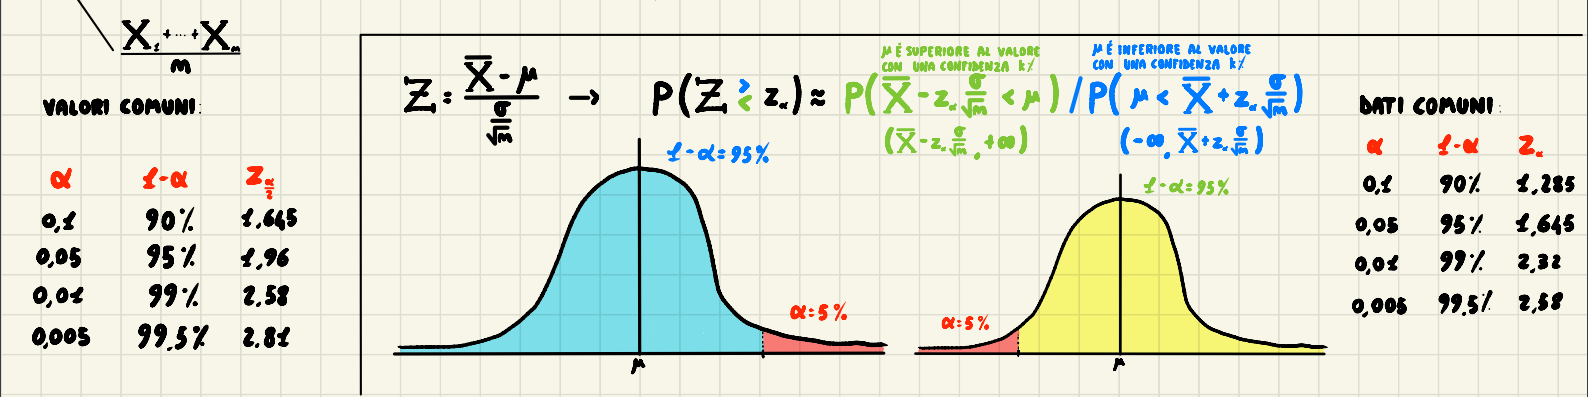
\includegraphics[width=\textwidth]{images/boh.png}
    \end{figure}
    \subsection{$\mu$ incognita e varianza  $\sigma^2$ incognita}
    Dato che tutti i nostri parametri sono ignoti, non possiamo basarci sul fatto che $\sqrt{n}(\overline{X} - \mu) / \sigma$ è una \textit{normale standard}, dobbiamo quindi ricorrere a una varianza campionaria come segue:
    \[ S^2 := \frac{1}{n-1} \sum_{i}^{} (X_i - \overline{X})^2 \longrightarrow \frac{\overline{X} - \mu}{\frac{S}{\sqrt{n}}} \sim t_{n-1}\]
    \centerline{Alla fine otteniamo una variabile aleatoria di tipo $t$ con n-1 gradi di libertà}
    \paragraph{Per Bilaterale}
    \[ P \left\{ \overline{X} - t_{\frac{\alpha}{2}, n-1} \frac{S}{\sqrt{n}} < \mu < \overline{X} + t_{\frac{\alpha}{2}, n_1} \frac{S}{\sqrt{n}} \right\} = 1 - \alpha \]
    \paragraph{Per Unilaterale}
    \[ P \left(  \overline{X} - t_{\frac{\alpha}{2}, n-1} \frac{\sigma}{\sqrt{n}} < \mu \right) / P \left( \mu < \overline{X} + t_{\frac{\alpha}{2}, n_1} \frac{\sigma}{\sqrt{n}}\right) = 1 - \alpha  \]
    \subsection{Metodo Montecarlo}
    supponendo di avere una funzione $f$ da $\mathbb{R}^r$ in $\mathbb{R}$ e vogliamo stimare la quantità $\theta$:
    \[ \theta := \int_{0}^{1} \int_{0}^{1} \cdots \int_{0}^{1} f(y_1, y_2, \ldots, y_n) \, dy_1 \, dy_2 \ldots \, dy_n \]
    Possiamo notare che $U_1, U_2, \ldots, U_r$ sono var. al. \textit{uniformi} su 0,1 quindi:
    \[ \ev{f(U_1, U_2, \ldots, U_r)} = \theta \]
    Se produciamo un numero casuale distribuito come la funzione e lo ripetiamo $n$ volte, possiamo stimare $\boldsymbol{\theta}$
    \[ \hat{\theta} = \frac{1}{n} \sum_{i = 1}^{n} X_i \]
    \paragraph{Esempio} pensiamo alla stima di questo integrale:
    \[ \theta := \int_{0}^{1} \sqrt{1 - y^2} \, dy = \ev{\sqrt{1-U^2}} \]
    Se $\boldsymbol{U_1, U_2, \ldots, U_{100}}$ sono variabili aleatorie con tale distribuzione e \textit{indipendenti} ponendo 
    \[ X_i := \sqrt{1-U^2_i} \qquad i = 1,2, \ldots, 100 \]
    Otteniamo un campione di \textbf{100} variabili aleatorie di media $\theta$. Calcoliamo ora la \textit{media campionaria}:
    \[ \hat{\theta} = \frac{1}{n} \sum_{i=1}^{n} X_1 = 0.786 \]
    e successivamente la \textit{deviazione standard campionaria}:
    \[ S = 0.23 \]
    dato che $t_{0.025, 99} \approx 1.985$ otteniamo che un intervallo di confidenza al 95\% per $\theta$ è il seguente:
    \[ 0.786 \pm 1.985 \cdot 0.023 \]
    \centerline{Quindi il valore è compreso tra 0.740 e 0.832}
    \section{Intervalli di predizione}
    \subsection{$\mu$ incognita e varianza $\sigma^2$ incognita}
    Supponiamo che $X_1, X_2, \ldots, X_n, X_{n+1}$ sia un campione normale di media $\mu$ e varianza $\sigma^2$ entrambe \textit{incognite}
    \[ \mu = \overline{X}_n = \frac{1}{n} \sum_{i = 1}^{n} X_i \sim \mathcal{N}(\mu, \frac{\sigma^2}{n})  \]
    \paragraph{Per la riproducibilità}
    \[ X_{n+1} - \overline{X}_n \sim \mathcal{N}(0, \sigma^2 + \frac{\sigma^2}{n}) \longrightarrow \frac{X_{n+1} - \overline{X}_n}{\sigma \sqrt{1+1 /n}} \]
    Dato che $\sigma$ è incognita dobbiamo sostituirla col suo stimatore (scegliendo la \textit{deviazione standard campionaria} quindi poniamo:
    \[ S^2_n := \frac{1}{n -1} \sum_{i= 1}^{n} (X_i - \overline{X}_n)^2 \]
    Questa grandezza è \textit{indipendente} da $\overline{X}_n$ quindi otteniamo
    \[ \frac{X_{n+1} - \overline{X}_n}{S_n \sqrt{1+1/n}} \sim t_n - 1 \]
    \paragraph{Esempio} prendiamo in campione i valori rilevati da un contapassi negli ultimi 7 giorni \\
    Dataset: 6822 5333 7420 6252 7005 6752 \\
    Si trovi l'intervallo di predizione al 95\% di confidenza \\
    \textbf{Risoluzione:} le statistiche del campione sono:
    \[ \overline{X}_7 \approx 6716.57 \qquad \qquad S_7 \approx 733.97 \]
    Dalle tabelle ricaviamo che $t_{0.025,6} \approx 2.447$ (+ altri passaggi) concludiamo col dire che il 95\% di confidenza che $X_8$ cadrà nell'intervallo [4796, 8637]
    \subsection{Intervalli do confidenza per la varianza} 
    Se $X_1, X_2, \ldots, X_n$ è un campione di una distribuzione \textit{normale} con parametri $\mu$ $\sigma^2$ \textbf{incogniti} ci possiamo basare sul fatto che
    \formula \[ (n-1) \frac{S^2}{\sigma^2} \sim \mathcal{X}^2_{n-1}  \]
    \paragraph{Per caso Bilaterale}:
    \begin{equation}
        \left(\frac{(n-1) s^2}{\chi_{\frac{\alpha}{2}, n-1}^2}, \quad \frac{(n-1) s^2}{\chi_{1-\frac{\alpha}{2}, n-1}^2}\right)
    \end{equation}
    \paragraph{Per caso Unilaterale}:
    \begin{equation}
        P \left( 0 < \sigma^2  < \frac{(n-1)S^2}{\mathcal{X}^2_{1-\alpha, n-1}}\right) / P \left( \frac{(n-1)S^2}{\mathcal{X}^2_{\alpha, n-1}} < \sigma^2 \right)
    \end{equation}
    \subsection{Stime per la differenza tra le medie di due popolazioni normali}
    Siano $X_1, X_2, \ldots, X_n$ e $Y_1, Y_2, \ldots, Y_m$ due campioni normali e differenti e denotiamo con $\mu_1$ e $\sigma^2_1$ e con $\mu_2$ e $\sigma^2_2$ \\
    $\boldsymbol{\overline{X} - \overline{Y}}$ è lo stimatore di massima verosomiglianza $\mu_1 - \mu_2$
    \begin{figure}[H]
        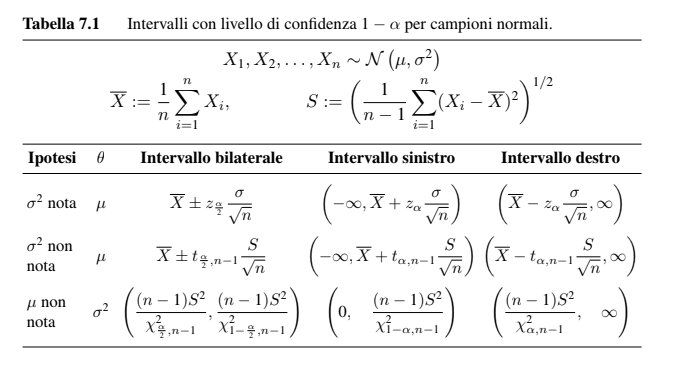
\includegraphics[width=\textwidth]{images/boh_2.png}
    \end{figure}
    Per ottenere uno \textit{stimatore non puntuale}, dobbiamo conoscere la distribuzione di $\overline{X} - \overline{Y}$ poiche:
    \[ \overline{X} \sim \mathcal{N} \left( \mu_1, \frac{\sigma^2_1}{n} \right)  \qquad e \qquad \overline{Y} \sim \mathcal{N}\left( \mu_2, \frac{\sigma^2_2}{m} \right) \]
    Possiamo dedurre che:
    \[ \overline{X} - \overline{Y} \sim \mathcal{N}\left( \mu_1 - \mu_2, \frac{\sigma^2_1}{n} + \frac{\sigma^2_2}{m} \right) \]
    Ipotizzando di conoscere $\sigma^2_1$ e $\sigma^2_2$ abbiamo che:
    \[ \frac{\overline{X} - \overline{Y} - (\mu_1 - \mu_2)}{\sqrt{\sigma^2_1 / n + \sigma^2_2 / m}} \sim \mathcal{N}(0,1) \]
    e possiamo dedurre, con i passaggi che ci sono ormai familiari, che
    \paragraph{Per caso Bilaterale}
    $$
    \begin{aligned}
    1-\alpha & =P\left(-z_{\frac{\alpha}{2}}<\frac{\overline{X}-\overline{Y}-\left(\mu_1-\mu_2\right)}{\sqrt{\sigma_1^2 / n+\sigma_2^2 / m}}<z_{\frac{\alpha}{2}}\right) \\
    & =P\left(\overline{X}-\overline{Y}-z_{\frac{\alpha}{2}} \sqrt{\frac{\sigma_1^2}{n}+\frac{\sigma_2^2}{m}}<\mu_1-\mu_2<\overline{X}-\overline{Y}+z_{\frac{\alpha}{2}} \sqrt{\frac{\sigma_1^2}{n}+\frac{\sigma_2^2}{m}}\right)
    \end{aligned}
    $$
    \paragraph{Per caso Unilaterale}
    $$
    \begin{aligned}
    1 - \alpha &= P\left( \overline{X} - \overline{Y} - z_{\alpha} \sqrt{\frac{\sigma^2_1}{n} + \frac{\sigma^2_2}{m} < \mu_1 - \mu_2} \right) / P \\
    &= \left( \mu_1 - \mu_2 < \overline{X} - \overline{Y} - z_{\alpha} \sqrt{\frac{\sigma^2_2}{n} + \frac{\sigma^2_2}{m}} \right)\\
    \end{aligned}
    $$
    \section{Intervalli di confidenza}
    \subsection{Intervalli approssimati per Bernoulli}



















    \[ P\{X_i = x\} = P^x (1-P)^x \quad x \in \{0, 1\} \]
    \centerline{Dove \textbf{X} è una \textit{variabile aleatoria} e \textbf{x} una \textit{variabile sperimentale} }
    \[ f(x_1 \ldots x_n / P) = P^{x_1} (1-P)^{1-x_1} \cdot P^{x_2} (1-P)^{1-x_2} \ldots P^{x_n} (1-P)^{1-x_n} = \]
    \[ P^{\sum_{i}^{n}x_i} (1-P)^{n - \sum_{1}^{n} x_i} \longrightarrow \text{Bisogna trovare il \textbf{massimo} della funzione} \]
    \begin{equation*}
        \begin{split}
            log(f(x_1 \ldots x_n / P)) &= \sum_{1}^{n} x_i log P - (n - \sum_{i}^{n} x_i) log(1-P) \\
            &= \frac{d}{dP}[log(f)] = 0 = \frac{1}{\hat{P}} \sum_{i}^{n} x_i - \frac{n - \sum_{i}^{} x_i }{(1-\hat{P})} \\
            &= (1- \hat{P}) \sum_{i}^{} x_i = \hat{P} (n - \sum_{i}^{} x_i) \\
            &= \hat{P} = \frac{\sum_{i}^{} x_i }{n} \quad \text{MLE}
        \end{split}
    \end{equation*}
    \paragraph{Esercizio 1} Probabilità che Oneto dia 30L (Lode) \\
    $n = 120$ \\
    $\sum_{i}^{120} x_i = 18$ \\
    $\hat{P} = \frac{18}{120} = 0.15 \rightarrow 15\%$ \\
    \paragraph{Esercizio 2} N studenti da 30 e lode \\
    $n_1 = 18 \leftarrow \text{Oneto}$ \\ 
    $n_2 = 20 \leftarrow \text{Anguita}$ \\
    $n_{1,2} = 10 \leftarrow \text{30L sia con Oneto che con Anguita}$ \\
    $N= ? \quad \text{Studenti da \textbf{30 e Lode}}$ \\
    \begin{minipage}{0.30\textwidth}
        \[ \hat{P_1} \approx \frac{n_1 2}{n_2} \]
    \end{minipage}
    \begin{minipage}{0.30\textwidth}
        \[ \hat{P_1} \approx \frac{n_1}{N} \]
    \end{minipage}
    \begin{minipage}{0.30\textwidth}
        \[ \frac{n_{1,2}}{n_2} = \frac{n_1}{N} \]
    \end{minipage} \\
    $ \Longrightarrow N= \frac{n_1 \cdot n_2}{n_{1,2}} \rightarrow \frac{18 \cdot 20}{10} = 36 $
    \paragraph{MLE POISSON}
    \begin{equation*}
        \begin{split}
            f(x_1, x_2 \ldots x_n / \lambda) &= \frac{e^{-\lambda} \lambda^{x_1}}{x_1 !} \cdot \frac{e^{-\lambda} \lambda^{x_2}}{x_2 !} \cdots \frac{e^{-\lambda} \lambda^{x_n}}{x_n !} \\
            &= \frac{e^{-n\lambda} \lambda^{\sum_{i}^{} x_i}}{x_1! x_2! \ldots x_n!}
        \end{split}
    \end{equation*}
    \formula
    $\lambda = \frac{\sum_{i}^{} x_i}{\lambda} \quad \text{MLE} $
    \paragraph{Esercizio 3} Stima del numero di incidenti medio in auto n = 10 \\
    $x_1 = \{ 4,0,6,5,2,1,2,0,4,3 \}$ \\
    $\hat{\lambda} = \frac{\sum_{i}^{} x_i}{n} = \frac{27}{10} = 2.7$
    \[ P\{x \leq 2 \} = e^{-2.7} (\frac{2.7^0}{0!} + \frac{2.7^1}{1!} + \frac{2.7^2}{2!}) \approx .4936 \rightarrow 49.36\% \]
    \centerline{Probabilità che non ci siano più di \textbf{2 incidenti} }
    \paragraph{MLE UNIFORME}
    \begin{equation*}
        f(x_1, x_2 \ldots x_n / \theta) =
        \begin{cases}
                \frac{1}{\theta^n} & \quad 0 < x_i < \theta \\
                0 & \quad \text{altrimenti}
        \end{cases}
    \end{equation*}
    $\hat{\theta} = \max\{x_i\}$ \\
    $\frac{\hat{\theta}}{2} = \frac{\max\{ x_i\}}{2}$
    \paragraph{MLE GAUSSIANA}
    \[ f(x_1,x_2 \ldots x_n / \mu, \sigma) = \prod_{i=1}^{n} \frac{1}{\sqrt{2\pi} \sigma} e^{\frac{-(x_1 - \mu)^2}{2 \sigma^2}} \]
    \[ (\frac{1}{2 \pi})^{\frac{n}{2}} \frac{1}{\sigma^n} e^{\frac{-\sum_{i}^{}(x_i - \mu)^2}{2 \sigma}} \]
    $log[f] = - \frac{n}{2} log 2\pi - n log \sigma - \frac{\sum_{i}^{}(x_i - \mu)^2}{2\sigma^2}$ \\ \\
    $\frac{d log f}{d \mu} = 0 = \frac{\sum_{i}^{}(x_i - \mu)^2}{\sigma^2} \longrightarrow \hat{\mu} = \frac{\sum_{i}^{}x_i}{n}$ \\
    $\frac{d log f}{d \sigma} = 0 = - \frac{n}{\sigma} + \frac{\sum_{i}^{} (x_i - \mu)^2}{4 \sigma^4} \rightarrow \sigma = \sqrt{\frac{\sum_{i}^{}(x_i - \mu)^2}{n}}$
    \paragraph{Esercizio} primo \\
    $x_1 = 1.7$ \\
    $x_2 = 1.82$ \\
    $x_3 = 1.73$\\
    $x_4 = 1.7$\\
    $x_5 = 1.8$ \\
    \[ \hat{\mu} = \frac{\sum_{i}^{} x_i}{n} = \frac{1.7 + 1.82 + 1.73 + 1.7 + 1.8}{5} = 1.75 \]
    \[ \hat{\sigma} = \sqrt{\frac{0.05^2 + 0.07^2 + 0.02^2 + 0.05^2 + 0.05^2}{5}} \approx 0.051 \]
    \paragraph{Intervalli di confidenza} normali
    TODO
    \paragraph{Intervalli di confidenza} gaussiani
    $\sigma^2$ Nota \\
    $x_1m x_2 \ldots x_n$ \\
    $\hat{\mu} \longleftarrow \mu$ \\
    $\frac{\overline{x} - \mu}{\frac{\sigma}{\sqrt{n}}} \sim \mathcal{N}(0,1)$ \\
    \[ P(-1.96 < \frac{\overline{x} - \mu}{\frac{\sigma}{\sqrt{n}}} < +1.96) = 0.95 \]
    \[ \longrightarrow P(-1.96 \frac{\sigma}{\sqrt{n}} < \overline{x} - \mu < 1.96 \frac{\sigma}{\sqrt{n}}) \]
    \[ P(\overline{x} - 1.96 \frac{\sigma}{\sqrt{n}} < \mu < \overline{x} + 1.96 \frac{\sigma}{\sqrt{n}}) \]
    \paragraph{Esempio:} Sistema di comunicazione
    $\sigma^2 = 4 \quad n = 9$
    \[ x_1 = \{ 5.85, 12, 15, 7, 9, 7.5, 6, 5, 10.5 \} \]
    \[ \hat{\mu} = \frac{1}{n} \sum_{i}^{n} x_i = \frac{1}{9} \sum_{i}^{n} x_i = \frac{81}{9} = 9 \] \\
    \begin{equation*}
        \begin{aligned}
            & P\left(9-1.96 \frac{\sigma}{\sqrt{m}}<\mu<9+1.96 \frac{\sigma}{\sqrt{m}}\right)=0.95 \\
            & p\left(9-1.96 \frac{2}{3}<\mu<9+1.96 \frac{2}{3}\right)=0.95 \\
            & \longrightarrow[7.693,10.31] \rightarrow \mu \text { si trova tra 7.693 e 10.31} \\
        \end{aligned}
    \end{equation*}
    \paragraph{In generale} Prob = $1-\alpha$
    \[ (\overline{x} - z_a \frac{\sigma}{\sqrt{n}}, \overline{x} + z_a \frac{\sigma}{\sqrt{n}} ) \rightarrow \text{Si rileva dalle tavole} \]
    \subsection{Intervalli di confidenza (Bilaterali)}
    \[ \overline{X} = \frac{1}{n} \sum_{i}^{n} x_i \]
    \[ x_i \sim \mathcal{N}(\mu, \sigma^2) \]
    \[ \overline{X} \sim(\mu, \frac{\sigma^2}{n}) \]
    \[ \mathcal{Z} = \frac{\overline{X} - \mu}{\frac{\sigma}{\sqrt{n}}} \sim \mathcal{N}(0, 1) \quad Var(\frac{x}{2}) = \frac{1}{\sigma^2} Var(x) \]
    \text{Supponiamo che $\sigma$ sia nota:}
    \begin{equation*}
        \begin{aligned}
            &\begin{aligned}
            & \operatorname{Pr}\left\{-z_{\frac{\alpha}{2}}<Z<+z_{\frac{\alpha}{2}}\right\}=1-\alpha \\
            & \operatorname{Pr}\left\{-z_{\frac{\alpha}{2}}<\frac{\bar{x}-\mu}{\frac{\sigma}{\sqrt{m}}}<+z_{\frac{\alpha}{2}}\right\}=1-\alpha \\
                & \operatorname{Pr}\left\{-z_{\frac{\alpha}{2}} \frac{\sigma}{\sqrt{m}}<\bar{x}-\mu<+z_{\frac{\alpha}{2}} \frac{\sigma}{\sqrt{m}}\right\}
        \end{aligned}\\
        &\begin{aligned}
        & \operatorname{Pr}\left\{-\bar{x}-z_{\frac{\alpha}{2}} \frac{\sigma}{\sqrt{m}}<-\mu<-\bar{x}+z_{\frac{\alpha}{2}} \frac{\sigma}{\sqrt{m}}\right\}= \\
        & \operatorname{Pr}\left\{\bar{x}-z_{\frac{\alpha}{2}} \frac{\sigma}{\sqrt{m}}<\mu<\bar{x}+z_{\frac{\alpha}{2}} \frac{\sigma}{\sqrt{m}}\right\}=1-\alpha
        \end{aligned}
        \end{aligned}
    \end{equation*}
    \subsection{Intervalli di confidenza (Unilaterali)}
    \begin{equation*}
        \begin{aligned}
        & \operatorname{Pr}\left\{z<z_\alpha\right\}=1-\alpha \\
        & \operatorname{Pr}\left\{\frac{\bar{x}-\mu}{\frac{\sigma}{\sqrt{m}}}<z_\alpha\right\}=1-\alpha \\
        & \operatorname{Pr}_r\left\{\bar{x}-\mu<z_\alpha \frac{\sigma}{\sqrt{m}}\right\}=1-\alpha \\
        & \operatorname{Pr}\left\{-\mu<-\bar{x}+z_\alpha \frac{\sigma}{\sqrt{m}}\right\}=1-\alpha \\
        & \operatorname{Pr}\left\{\bar{x}-z_\alpha \frac{\sigma}{\sqrt{m}}<\mu\right\}=1-\alpha \\
        & \mu \in\left(\bar{x}-z_\alpha \frac{\sigma}{\sqrt{m}},+\infty\right)
        \end{aligned}
    \end{equation*}
    \subsection{Esempio:} Pesca stagionale dei salmoni (\textit{Fisso intervallo -> trovo $n$}) \\
    \text{Ad ogni stagione il peso medio dei salmoni è diverso ma $\sigma = 0.3$ Kg} \\
    \text{Intervallo di confidenza al 95\%, quindi $\alpha = 0.05$}
    \[ (\overline{X} - 1.96 \frac{\sigma}{\sqrt{n}}, \overline{X} + 1.96 \frac{\sigma}{\sqrt{n}}) \]
    \[ 1.96 \frac{\sigma}{\sqrt{n}} \geq 0.1 \quad \sqrt{n} \geq \frac{1.96}{0.1} \sigma \]
    \[ n \geq (\frac{1.96}{0.1} 0.3)^2 = 5.88^2 \approx 34.6 \leftarrow \text{salmoni} \]
    \subsection{Intervallo di confidenza} con \textit{media} e \textit{varianza} \textbf{incognite}
    \begin{equation*}
        \begin{aligned}
            & Z=\frac{\bar{x}-\mu}{\frac{\sigma}{\sqrt{n}}} \sigma \quad \text{ Non nota} \\
            & s^2=\frac{1}{n-1} \sum_i\left(x_i-\bar{x}\right)^2=\frac{1}{n-1} \sum_i^n\left(x_i^2-n \bar{x}^2\right) \\
            & =\frac{1}{n-1} \sum_i\left(x_i^2+\bar{x}^2-2 x_i \bar{x}\right) \\
            & =\frac{1}{n-1} \sum_i x_i^2+\frac{n \bar{x}^2}{n-1}-2 \bar{x} \frac{\bar{x} n}{n-1} \\
        \end{aligned}
    \end{equation*}
    \[ T = \frac{\overline{X} - \mu}{\frac{s}{\sqrt{n}}} \sim T_n - 1 \quad \text{(T studenti con n gradi di libertà)} \]
    \paragraph{Esempio:} Trasimttente ($\mu$) e ricevitore ($\mu$ + rumore)
    \[ 95\% (7.69, 10.31) \quad \hat{\mu} = 9, \sigma^2 = 4 \]
    $X_i \{ 5, 8.5, 12, 15, 7, 9, 7.5, 6.5, 10.5 \}$ \\
    $\hat{\mu} = \overline{X} = \frac{1}{9} \sum_{i}^{n} X_i = \frac{81}{9} = 9$ \\
    $s^2 = \frac{1}{8}\sum_{i}^{}(X_i^2-9.81) \approx 9.5 \quad s = 3.082$
    \[ \mu \in (9-2.306 \frac{3.082}{3}, 9 + 2.306 \frac{3.082}{3}) = (6.63, 11.37) \]
    \centerline{Si può dimostrare che $T_{\frac{\alpha}{2} \cdot n - 1} \ev{S} \geq z_\alpha\sigma$}
    \subsection{Integrali Monte Carlo}
    \[ \theta = \ev{f(u)} = \int_{-\infty}^{+\infty} f(u) p(u) \, du = \int_{-\infty}^{+\infty} f(u) \, du \]
    \paragraph{Esempio}: \\
    $\int_{0}^{1} \sqrt{1-x^2} \,dx = ?$
    $\ev{\sqrt{1-x^2}} \quad n = 100$ \\
    $X_i = \sqrt{1 - U_i^2} \quad X = \{ X_1, X_2 \ldots X_100 \}$ \\
    $\hat{\theta} = \overline{X} \pm t_{\frac{\alpha}{2}}, 99 \frac{s}{\sqrt{100}} \rightarrow \text{Per vedere se il risultato è corretto \textit{(confidenza)}}$ 
    \subsection{Intervallo di confidenza di Bernoulli}
    n esperimenti \\
    Binomiale \\
    media np \\
    varianza np(1-p) \\
    \[ \hat{P} = \frac{1}{n} \sum_{i}^{n}X_i \quad X_i \in \{ 0, 1 \} \] \\
    \[ X = n\hat{P} \quad P_r \{ -z_{\frac{\alpha}{2}} < z < z_{\frac{\alpha}{2}} \approx 1-\alpha \}\] \\
    \centerline{Dove z = $\frac{X-np}{\sqrt{np(1-p)}}$}
    \[ \frac{x-nP}{\sqrt{nP(1-P)}} \sim \mathcal{N}(0,1)\]
    \begin{equation}
        \begin{aligned}
        & \rho_r\left\{-z_{\frac{a}{2}}<\frac{x-m p}{\sqrt{m p(1-\hat{p})}}<z_{\frac{a}{2}}\right\} \cong 1-\alpha \\
        & \rho_r\left\{\hat{p}-z_{\frac{a}{2}} \sqrt{\frac{p(1-p)}{m}}<\mu<\hat{p}+z_{\frac{\alpha}{2}} \sqrt{\frac{\hat{p}(1-p)}{m}}\right\} \simeq 1-\alpha
        \end{aligned}
    \end{equation}

    \section{Intervalli di confidenza}
    \paragraph{Se $\sigma^2$ è nota} allora:
    \[ X_i \sim \mathcal{N}(\mu, \sigma^2) \quad \overline{X} = \frac{1}{n} \sum_{i}^{n} X_i \]
    \begin{equation*}
        \begin{aligned}
            \mu \in (-\infty, \overline{X} + z_\alpha \frac{\sigma}{\sqrt{n}}) \\
            \mu \in (\overline{X} - z_{\frac{\sigma}{\sqrt{n}}}, \overline{X} + z_{\frac{\sigma}{\sqrt{n}}}) \quad p_r (1-\alpha) \\
            \mu \in (-\infty, \overline{X} + z_\alpha \frac{\sigma}{\sqrt{n}}) \\
            \mu \in (\overline{X} - z_\alpha \frac{\sigma}{\sqrt{n}}, \infty)
        \end{aligned}
    \end{equation*}
    $s^2 = \frac{1}{n - 1} \sum_{i}{} (X_i - \overline{X})$ \\
    Se $\sigma^2$ è ignota allora: \\
    \[ \mu \in (\overline{X} - z_{\frac{\alpha}{2}}, n - 1 \frac{s}{\sqrt{n}}) \quad \sigma^2 \rightarrow s^2 = z \rightarrow t \]
    \subsection{Intervallo di confidenza nella varianza}
    \[ (n-1) \frac{S^2}{\sigma^2} \sim \mathcal{X}^2 \quad X_i \sim \mathcal{N}(\mu, \sigma^2) \]
    \begin{equation*}
        \begin{aligned}
            p_r \left \{ \mathcal{X}_{1- \frac{\alpha}{2}, n - 1}^2 \leq (n-1)\frac{s^2}{\sigma^2} \leq \mathcal{X}_{\frac{\alpha}{2}, n-1} \right \} \\
            p_r \left \{ \frac{s^2(n-1)}{\mathcal{X}_{\frac{\alpha}{2}, n-1}} \leq \sigma^2 \leq \frac{s^2(n-1)}{\mathcal{X}_{1- \frac{\alpha}{2}, n - 1}^2} \right \} = 1-\alpha \\
            \sigma^2 \in \left (\frac{s^2(n-1)}{\mathcal{X}_{\frac{\alpha}{2}, n-1}^2}, \frac{s^2(n-1)}{\mathcal{X}_{1- \frac{\alpha}{2}, n-1}}\right )  \quad p_r = 1- \alpha
        \end{aligned}
    \end{equation*}
    \paragraph{Esempio:} Laminatoio n = 4
    $X_i = \{ 0.123, 0.124, 0.126, 0.12 \} \text{spessore in \textbf{mm}}$ \\
    \paragraph{Svolgimento}
    \begin{equation*}
        \begin{aligned}
            \frac{1}{4} \sum_{i}^{4} X_i = \frac{0.493}{4} = 0.12325 \\
            \frac{1}{4-1} \sum_{i}^{4}\left ( X_i - 0.12325 \right )^2 = 1.875 \cdot 10^{-5} \\
            \sigma^2 \in \left ( \frac{s^2(n-1)}{9.348}, \frac{s^2(n-1)}{0.216} \right )
        \end{aligned} 
    \end{equation*}
    \centerline{Dove \textbf{9.348} e \textbf{0.216} sono ricavati dalle tabelle}
    Facciamo la radice: \\
    $\sigma \in (0.0014, 0.0093) \rightarrow 95\% $
    \subsection{Intervallo di confidenza}della differenza di due medie: \\ \\
    \begin{minipage}{0.5\textwidth}
        \centerline{\textbf{N} campioni}
        \[ X_i \sim \mathcal{N}(\mu_1, \sigma_1^2) \]
        \[ \overline{X} = \frac{1}{n} \sum_{i}^{n} X_i \]
    \end{minipage}
    \begin{minipage}{0.5\textwidth}
        \centerline{\textbf{M} campioni}
        \[ Y_i \sim \mathcal{N}(\mu_2, \sigma_2^2) \]
        \[ \overline{Y} = \frac{1}{m} \sum_{i}^{m} Y_i \]
    \end{minipage}
    \[ \overline{X} - \overline{Y} \sim \mathcal{N}\left ( \mu_1 - \mu_2, \frac{\sigma_1^2}{n} + \frac{\sigma_2^2}{m} \right ) \]
    \[ \mathcal{N}(0,1) \sim \frac{\overline{X} - \overline{Y} - (\mu_1 - \mu_2)}{\sqrt{\frac{\sigma_1^2}{n} + \frac{\sigma_2^2}{m}}} \]
    $\mu_1 - \mu_2 \in \left ( \overline{X} - \overline{Y} - z_{\frac{\alpha}{2}} \sqrt{\frac{\sigma_1^2}{n} + \frac{\sigma_2^2}{m}}, \overline{X} - \overline{Y} + z_{\frac{\alpha}{2}}, \overline{X} - \overline{Y} + z_{\frac{\alpha}{2}} \sqrt{\frac{\sigma_1^2}{n} + \frac{\sigma_2^2}{m}} \right )$ \\ \\
    Se $\sigma_1^2, \sigma_2^2$ non sono note: \\ \\
    \begin{minipage}{0.5\textwidth}
        $S_1^2 = \frac{1}{n-1} \sum_{i}^{n}(X_i - \overline{X})$ \\ \\
        $(n-1) \frac{S_1^2}{\sigma_1^2} \sim \mathcal{X}_{n-1}^2$
    \end{minipage}
    \begin{minipage}{0.5\textwidth}
        $s_2^2 = \frac{1}{m - 1} \sum_{i}^{m} (X_i - \overline{Y})$ \\ \\
        $(n-1) \frac{s_2^2}{\sigma_2^2} \sim \mathcal{X}_{n-1}^2$
    \end{minipage} \\ \\
    \textbf{Possiamo andare avanti solo se \boldsymbol{$\sigma_1^2 = \sigma_2^2 = \sigma^2$}}
    \[ (n-1) \frac{s_1^2}{\sigma^2} + (n-1) \frac{s_2^2}{\sigma^2} \sim \mathcal{X}_{n+m-2}^2 \]
    \[ \frac{\overline{X} - \overline{Y} - (\mu_1 - \mu_2)}{\sqrt{\sigma^2 (\frac{1}{n} + \frac{1}{m})}} \longrightarrow \frac{\overline{X} - \overline{Y} - (\mu_1 - \mu_2)}{\sqrt{S_p(\frac{1}{n} + \frac{1}{m})}} \]
    \[ \sim \mathcal{N}(0,1) \quad \quad \quad \quad \quad \sim T_{n+m-2}\]
    $S_p = \frac{(n-1) S_1^2 + (m-1) S_2^2}{n+m-2}$ \\ \\
    \centerline{Se $\sigma$ sono ignote ma uguali}
    $\mu_1 - \mu_2 \in (\overline{X} - \overline{Y} -T_{\frac{\alpha}{2},n+m-2} \sqrt{s^2(\frac{1}{n} + \frac{1}{m})})$ \\
    $\overline{X} - \overline{Y} + T_{\frac{\alpha}{2}, n+m-2} \sqrt{s^2 (\frac{1}{n} + \frac{1}{m})}$
    \subsection{Intervallo di previsione}
    $X_1, \ldots X_n, X_{n+1} \sim \mathcal{N}(\mu, \sigma^2)$ \\
    $\overline{X}_n = \frac{1}{n} \sum_{i}^{n} X_i \quad \overline{X}_n \sim \mathcal{N}(\mu, \frac{\sigma^2}{n})$ \\
    $\overline{X}_n - X_{n+1} \sim \mathcal{N}(0, \sigma^2 + \frac{\sigma^2}{n}) \rightarrow (\mu - \mu, \sigma^2 + \frac{\sigma^2}{n})$ \\
    $\sigma^2(1 + \frac{1}{n})$
    \begin{minipage}{0.4\textwidth}
        $\frac{X_n - X_n + 1}{\sigma \sqrt{1 + \frac{1}{n}}} \sim \mathcal{N}(0,1)$
    \end{minipage}
    \begin{minipage}{0.4\textwidth}
        $s_n^2 = \frac{1}{n-1} \sum_{i}^{} (X_i - \overline{X}_n)^2$
    \end{minipage}
    \[ X_{n+1} \in(\overline{X}_n - T_{\frac{\alpha}{2}, n-1} s_n \sqrt{1 + \frac{1}{n}}, \overline{X}_n + T_{\frac{\alpha}{2}, n-1} s_n \sqrt{1 + \frac{1}{n}}) \longrightarrow P_r(1-\alpha) \]
    \paragraph{Esempio} smartwatch contapassi $\boldsymbol{n = 7}$ \\ \\
    \centerline{\begin{minipage}{0.3\textwidth}
        $LUN \quad 6922 \quad X_1$ \\
        $MAR \quad 5333 \quad X_2$ \\
        $MER \quad 7420 \quad X_3$ \\ 
    \end{minipage}
    \begin{minipage}{0.3\textwidth}
        $GIO \quad 7432 \quad X_4$ \\
        $VEN \quad 6252 \quad X_5$ \\
        $SAB \quad 7005 \quad X_6$ \\
    \end{minipage}} \\
    \[ DOM \quad 6752 \quad X_7 \]
    \[ \overline{X}_n = \frac{1}{n} \sum_{i}^{m} X_i = \frac{47016}{7} \approx 6717 \]
    \[ 1-\alpha = 95\% \quad \alpha = 5\% \]
    \[ t_{0.0025,6} = 2.997 \]
    \[ S_n = \sqrt{S_n^2} = 7.333.8 \]
    \[ x_{n+1} \in (6717 -2.447 \cdot 733397 \sqrt{1 + \frac{1}{7}}, 6717 + 2.447 \cdot 73397 \sqrt{1 + \frac{1}{7}}) \]
    $X_{n+1} \in (9796, 8637) \mu \in (6037, 7396)$
    \subsection{Qualità di uno stimatore}
    $X = X_1 \ldots X_n \quad \theta \leftarrow \text{parametro} \quad \quad d(x) \leftarrow \text{stimatore di $\theta$}$ \\
    \begin{minipage}{0.5\textwidth}
        \[ \boldsymbol{(d(x) - \theta)^2}\] Errore Quadratico (\textit{misura della qualità})
    \end{minipage}
    \begin{minipage}{0.5\textwidth}
        \[ \boldsymbol{\ev{(d(x)-\theta)^2}} \] Errore Quadratico Medio (\textit{M.S.E})
    \end{minipage} \\
    Rischio $r(d, \theta) = \ev{(d-\theta)^2}$ 
    Lo stimatore "ottimo" sarà quello con il rischio minimo -> d con r minimo $\theta$
    \paragraph{Esempio}
    $d^* (x) = 4 \quad \text{se} \theta = 4 \Rightarrow d^* = \text{stimatore ottimo(per tutti gli altri valori non va bene)}$
    \subsection{Proprietà di uno stimatore}
    Def: $b_\theta(d) = \ev{d} - \theta \rightarrow \text{bias o polarizzazione}$
    Uno stimatore non è \textbf{polarizzato} se $b_\theta(d) = 0$
    \paragraph{Esempio}:
    $X_1 \ldots X_n \quad \theta \text{media}$ \\
    $d_1(X_1 \ldots X_n) = X_1$ \\
    $d_2(X_1 \ldots X_n) = \frac{X_1 + X_2}{2}$ \\
    $d_3(X_1 \ldots X_n) = \frac{X_1 + X_2 + \ldots X_n}{n}$
    \centerline{Tutti questi sono \textbf{unbiased}}
    \subsection{Stimatore unbaieseo}
    $r(d, \theta) = \ev{(d(x) - \theta)^2} = \ev{(d(x) - \ev{d(x)})^2} = Var(d)$ \\
    tra gli stimatori non polarizzati di ottimo è quello con la varianza minima
    \subsection{Valutazione di uno stimatore}
    \[ X = X_1 \ldots X_n \quad \theta = ? \]
    \centerline{Dove $\theta$ è un \textit{parametro} e $d(x)$ è uno \textit{stimatore} di $\theta$} \\ \\
    $r(d, \theta) \text{(mse) rischio} \quad \quad b_\theta(d) = \ev{d} - \theta$ \\
    se $b_\theta(d) = 0 \Rightarrow r(d, \theta) = Var(d)$ \\
    \centerline{se $b_\theta(d) \not = 0$ ? $r(d, \theta)$ = ?}
    \begin{equation*}
        \begin{split}
            r(d, \theta) = \ev{(d(x) - \theta)^2} &= \ev{(d(x) - \ev{d} + \ev{d} - \theta)^2} \\
            &= \ev{(d - \ev{d})^2 + (\ev{d} - \theta)^2 - 2(d - \ev{d}) (\ev{d} - \theta)} \\
            &= \ev{(d - \ev{d})^2} + \ev{(\ev{d} - \theta)^2} - 2(\ev{d} - \theta) \cdot \ev{(d- \ev{d})}
        \end{split}
    \end{equation*}
    \begin{equation*}
        \begin{split}
           r(d, \theta) &= \ev{(d - \ev{d})^2} + \ev{(\ev{d} - \theta)^2} \\
           &= Var(d) + b_\theta(d)^2 \leftarrow \text{bias$^2$}
        \end{split}
    \end{equation*}
    \subsection{Esempio:} Stimatore della media di una \textit{distribuzione uniforme} \\\\
    \begin{minipage}{0.4\textwidth}
        $\ev{X_i} = \theta / 2$ \\
        $X_1, X_2 \ldots X_n$
    \end{minipage}
    \begin{minipage}{0.4\textwidth}
        $d_1 = 2 \frac{1}{n} \sum_{i}^{n} X_i$ \\
        $d_2 = \max X_i$
    \end{minipage} \\[4ex]
    $d_1 : \ev{d_1} = \frac{2}{n} \sum_{i}^{} \ev{X_i} = \frac{2}{n} n \frac{\theta}{2} = \theta$ \\
    $r(d_1, \theta) = Var(d_1) = \frac{4}{n^2} n Var(X_i) = \frac{4}{n} \frac{\theta^2}{12} = \boldsymbol{\frac{\theta^2}{3n}} \Leftarrow$ \textit{Unbiased} \\[4ex]
    \begin{equation*}
        \begin{split}
            F_2(x) = P_r \{ d_2(x) \leq x \} &= P_r \{ \max X_1 \leq x \} \\
            &= P_r \{ X_1 \leq, \forall i \in 1 \} = \prod_{i = 1}^{n} P_r \{ X_i \leq x \} = (\frac{x}{\theta})^n \\
            f_2(x) &= \frac{d}{dx} F_2(x) = n \frac{x^{n-1}}{\theta^n} \quad x \leq \theta
        \end{split}
    \end{equation*} \\[6ex]
    $\displaystyle \ev{d_2} = \int_{0}^{\theta} x f_x(x) \, dx = \int_{0}^{\theta} \frac{n}{\theta^n} x^n \, dx = \frac{n}{\theta^n} \left[ \frac{x^{n+1}}{n+1} \bigg\rvert_{0}^{\theta}\right] = \frac{n}{n+1} \theta$ \\[2ex]
    $\displaystyle \ev{d_2^2} = \frac{n}{\theta^n} \int_{0}^{\theta} x^2 f(x) \, dx = \frac{n}{\theta^n} \int_{0}^{\theta} x^{n+1} \, dx = \frac{n}{\theta^n} \left[ \frac{x^{n+2}}{n+2} \bigg\rvert_{0}^{\theta}\right] = \frac{n}{n+2} \theta^2$ \\[2ex]
    $Var(d_2) = \ev{d^2} - \ev{d_2}^2 = \frac{n}{n+2}\theta^2 - \frac{n^2}{(n+1)^2} \theta^2 = \boldsymbol{\frac{n}{(n+2)(n+1)^2} \theta^2}$ \\[4ex]
    $r(d_2, \theta) = Var(d_2) + (\ev{d_2} - \theta)^2 = \boldsymbol{\frac{2 \cdot \theta^2}{(n+1)(n+2)}}$ \\[4ex]
    $n \geq 4 \quad r(d_2, \theta) < r(d_1, \theta) \quad \quad d_3 = \frac{n+1}{n} d_2$

    \paragraph{In sintesi}
    \begin{equation*}
        \begin{aligned}
            r(d_1, \theta) = \frac{\theta^2}{3n} \Leftarrow \text{Unbiased} \\
            r(d_2, \theta) = \frac{2\theta^2}{(n+1)(n+2)} \Leftarrow \text{Biased} \\
            r(d_3, \theta) = \frac{\theta^2}{n^2 + 2n} \Leftarrow \text{Unbiased} \\
            r(d_4, \theta) = \frac{\theta^2}{(n+1)^2} \Leftarrow \text{Biased}
        \end{aligned}
    \end{equation*}
    \section{Test di ipotesi}
    \paragraph{Ipotesi:} Affermazione rispetto a uno o più parametri di una distribuzione
    Ipotesi da confutare: $H_0$ (ipotesi nulla) \\
    \paragraph{Esempio}:
    \begin{equation}
        \begin{aligned}
            X_1 \ldots X_n \sim \mathcal{N}(\mu, \sigma^2) \\
            H_0 : \mu = 0 \\
            H_a : \mu \not = 0
        \end{aligned}
    \end{equation}
    \centerline{Diamo per scontato che l'ipotesi sia \textbf{vera}}
    \centerline{Dobbiamo cercare di \textit{confutarla}}
    \paragraph{Definizione} Regione critica tale che: \\\\
    $(X_1 \ldots X_n) \in C \rightarrow H_0 \text{è rifiutata}$ \\
    $(X_1 \ldots X_n) \not\in C \rightarrow H_0 \text{è accettata}$ \\
    $\alpha = $ Livello di \textbf{significatività} del test ($\alpha = 10\%, 5\% \ldots$)
    \paragraph{Procedimento}
    \begin{itemize}
        \item Fisso alpha
        \item Suppongo che $\alpha$ sia vera
        \item calcolo stima di $\mu$
        \item verifico che non sia "\textit{troppo distante}"
    \end{itemize}
    $X_1 \ldots X_n \sim \mathcal{N}(\mu, \sigma^2)$ \\
    $H_0 : \mu = \mu_0 \quad H_a : \mu \not = \mu_0$ \\
    $\overline{X} = \frac{1}{n} \sum_{i}^{} X_i $
    \paragraph{Regione critica}
    $\{ (X_1 \ldots X_n): \rvert \overline{X} - \mu_0 \rvert > c \}$ \\
    $P_{r_{\mu_0}} \left\{ | \overline{X} - \mu_0 | > c \right\} = \alpha$ \\
    $P_{r_{\mu_0}} \left\{ \frac{|\overline{X} - \mu_0|}{\frac{\sigma}{\sqrt{n}}} > \frac{c}{\frac{\sigma}{\sqrt{n}}} \right\} = \alpha$ \\
    $P_{r_{\mu_0}} \left\{ |z| > z_\alpha \right\} = \alpha$
    \paragraph{Esempio} (5 transimissioni) \\
    \begin{minipage}{0.45\textwidth}
        $\boldsymbol{n=5}$ \\
        $\overline{X} = 9.5$
    \end{minipage}
    \begin{minipage}{0.45\textwidth}
        $H_0 : \mu = 8$ \\
        $\alpha = 5\%$
    \end{minipage} \\[4ex]
    Ipotizzando che $H_0$ sia vera:
    \[ \frac{|\overline{X} - \mu|}{\frac{\sigma}{\sqrt{n}}} = \frac{|9.5 - 8|}{\frac{2}{\sqrt{5}}} \approx 1.68 \]
    Se: \\
    $\alpha = P_r$(rifiuto $H_0$ / $H_0$ vera) \\
    $\alpha \uparrow$ più \textit{"facile"} rifiutare l'ipotesi \\
    $\alpha \downarrow$ più \textit{"difficile"} rifiutare l'ipotesi
    \subsection{Metolodogia alternativa}
    \[ Ts = \frac{\overline{X} - \mu_0}{\frac{\sigma}{\sqrt{n}}} \rightarrow \text{Statistica di test} \]
    $P-$value = \textbf{probabilità} di ottenere un valore più "anomalo" di quello osservato
    \paragraph{Esempio:} $X_i \sim \mathcal{N}(\mu, 4)$ \\
    \begin{minipage}{0.5\textwidth}
        \[ n = 5 \]
        \[ \overline{X} = 8.5\]
    \end{minipage}
    \begin{minipage}{0.5\textwidth}
        \[ H_0 : \mu = 8 \]
        \[ H_a : \mu \not = 8\]
    \end{minipage}
    \[ \frac{|\overline{X} - \mu_0|}{\frac{\sigma}{\sqrt{n}}} = \frac{|8.5 - 8|}{\frac{2}{\sqrt{5}}} = \frac{\sqrt{5}}{2} 0.5 \approx 0.559 \]
    \[ P \{ |z| > 0.559 \} = 2P \{ z > 0.559 \} \approx 2 \cdot 0.288 = 0.579 \rightarrow \text{P-value}\] \\[2ex]
    Se $\boldsymbol{\overline{X} = 11.5}$:
    \[ \frac{|\overline{X} - \mu_0|}{\frac{\sigma}{\sqrt{n}}} = \frac{|11.5 - 8|}{\frac{2}{\sqrt{5}}} \approx 3.913 \]
    \[ P \{ |z| > 3.913 \} = 2P \{ z > 3.913 \} \leq 0.00005 \rightarrow \text{\underline{Rifiuto ipotesi $H_0$}}\]
    \subsection{Test di Hp unilaterale}
    \begin{minipage}{0.5\textwidth}
        \[ H_0 : \mu = \mu_0 (\mu \leq \mu_0) \]
    \end{minipage}
    \begin{minipage}{0.5\textwidth}
        \[ H_a : \mu > \mu_0 \]
    \end{minipage}
    \[ C = \{ (X_1 \ldots n) \cdot \overline{X} - \mu_0 > c \} \]
    \[ P_{r_{\mu_0}} \{ \overline{X} - \mu_0 > c \} = P_r \{ \frac{\overline{X} - \mu_0}{\frac{\sigma}{\sqrt{n}}} > \frac{c}{\frac{\sigma}{\sqrt{n}}}\} = P_{r_{\mu_0}} \{ z > z_a \} = \alpha \] \\[2ex]
    \centerline{Statistica test $\boldsymbol{\frac{\overline{X} - \mu_0}{\frac{\sigma}{\sqrt{n}}} \leq z_\alpha}$ accetto}
    \subsection{Test di ipotesi}
    \begin{minipage}{0.2\textwidth}
        $H_0$ \\[2ex]
        $\mu = \mu_0$
    \end{minipage}
    \begin{minipage}{0.2\textwidth}
        $H_a$ \\[2ex]
        $\mu \not= \mu_0$
    \end{minipage}
    \begin{minipage}{0.2\textwidth}
        TS \\[2ex]
        $\frac{\overline{X} - \mu_0}{\sigma / \sqrt{1}}$
    \end{minipage}
    \begin{minipage}{0.2\textwidth}
        Livello $\alpha$ \\[2ex]
        Rifiuto $H_0$ \\
        se $TS > \frac{z\alpha}{2}$
    \end{minipage}
    \begin{minipage}{0.2\textwidth}
        P - Value \\[2ex]
        $2P(z \geq |TS|)$
    \end{minipage}
    \paragraph{Altre ipotesi}: \\[2ex]
    \begin{minipage}{0.2\textwidth}
        $H_0$ \\[2ex]
        $\mu < \mu_0$ \\
        $\mu \geq \mu_0$
    \end{minipage}
    \begin{minipage}{0.2\textwidth}
        $H_a$ \\[2ex]
        $\mu > \mu_0$ \\
        $\mu < \mu_0$
    \end{minipage}
    \begin{minipage}{0.2\textwidth}
        TS \\[2ex]
        $\frac{\overline{X} - \mu_0}{\sigma / \sqrt{2}}$ \\
        \textit{//}
    \end{minipage}
    \begin{minipage}{0.2\textwidth}
        Livello $\alpha$ \\[2ex]
        $H_0 \quad z_\alpha > TS$ \\
        $H_0 \quad z_\alpha < -TS$
    \end{minipage}
    \begin{minipage}{0.2\textwidth}
        P - Value \\[2ex]
        $P(z\geq TS)$ \\
        $P(z \leq TS)$
    \end{minipage}
    \subsection{Uguaglianza media di due popolazioni}
    \begin{minipage}{0.45\textwidth}
        $X_1 \ldots X_n \sim \mathcal{N}(\mu_1, \sigma_2^2)$ \\
        $\overline{X} = \frac{1}{n} \sum_{i}^{n} X_i$ \\
        $S_x^2 = \frac{1}{n - 1} \sum_{i}^{} (X_i - \overline{X})^2$
    \end{minipage}
    \begin{minipage}{0.45\textwidth}
        $Y_i \ldots Y_m \sim \mathcal{N} (\mu_2, \sigma_2^2)$ \\
        $\overline{Y} = \frac{1}{m} \sum_{i}^{m} Y_i$ \\
        $S_y^2 = \frac{1}{m-1} \sum_{i}^{} (Y_i - \overline{Y})^2$
    \end{minipage}
    \[ S_p^2 = \frac{(n-1)S_x^2 + (m-1)S_y^2}{n+m} \]
    \begin{minipage}{0.2\textwidth}
        $H_0$ \\[2ex]
        $\mu_1 = \mu_2$ \\[2ex]
        $\mu_1 = \mu_2$ \\[2ex]
        $\mu_1 = \mu_2$
    \end{minipage}
    \begin{minipage}{0.2\textwidth}
        $H_a$ \\[2ex]
        $\mu \not =  \mu_2$ \\[2ex]
        $\mu \not =  \mu_2$ \\[2ex]
        $\mu \not =  \mu_2$
    \end{minipage}
    \begin{minipage}{0.2\textwidth}
        TS \\[2ex]
        $\frac{\overline{X} - \overline{Y}}{\sqrt{\sigma^2_{1/n} + \sigma^2_{2/m}}}$ \\[2ex]
        $\frac{\overline{X} - \overline{Y}}{\sqrt{S_p^2(\frac{1}{n} + \frac{1}{m})}}$ \\[2ex]
        $S_i \in \text{T-student}$ 
    \end{minipage}
    \begin{minipage}{0.2\textwidth}
        Livello $\alpha$ \\[2ex]
        rif. $|TS| > z_{\frac{\alpha}{2}}$
    \end{minipage}
    \begin{minipage}{0.2\textwidth}
        P - Value \\[2ex]
        $2P(z\geq |TS|)$
    \end{minipage} 
    \paragraph{4) T-test per coppie di dati}
    Se $X_1$ e $X_2$ \underline{\textbf{NON}} sono indipendenti \\
    \begin{minipage}{0.5\textwidth}
        $W_i = X_i - Y_i$
    \end{minipage}
    \begin{minipage}{0.5\textwidth}
        $X_i \sim \mathcal{N}(\mu_1, \sigma_1^2)$ \\
        $Y_i \sim \mathcal{N}(\mu_2, \sigma_2^2)$
    \end{minipage}
    \paragraph{ES} Manutenzione (n guasti) tagliand \\[2ex]
    $H_0 : \mu_a - \mu_b \geq 0 \quad \overline{W} = \frac{1}{5}(-7.5 + 2.5 - 2.5 - 3.5 -1.5) = -2.5$ \\[2ex]
    $S^2_W = \frac{1}{4}(W_i - \overline{W})^2 = 13$ \\[2ex]
    $Ts = \frac{\frac{\overline{W}}{S_W}}{\sqrt{n}} = \frac{\frac{-2.5}{\sqrt{13}}}{\sqrt{5}} = 1.55$
    \[ P_r \{ T_{n-1} \leq Ts \} = \{ T_4 \leq Ts \}\]
    \paragraph{5) Test sulla varianza}
    \[ H_0 : \sigma^2 = \sigma^2_0 \quad H_a : \sigma^2 \not = \sigma^2_0 \]
    \[ \frac{(n-1)}{\sigma^2_0} \sim \mathcal{X}^2_{n-1} \]
    $Pr \{ \mathcal{X}^2_{1-\frac{\alpha}{2}, n-1} \leq \frac{(n-1) s^2}{\sigma^2_0} \leq \mathcal{X}^2_{\frac{\alpha}{2}, n-1}\} = 1 -\alpha$
    \paragraph{Uguaglianza di varianza}: \\
    $X_1 \ldots X_n \qquad Y_1 \ldots Y_n \quad H_0 : \sigma^2_x = \sigma^2_y \qquad H_a : \sigma^2_x \not = \sigma^2_y$ \\[2ex]
    $\displaystyle S^2_x - S^2_y \quad Ts = \frac{\frac{S^2_x}{\sigma^2_x}}{\frac{S^2_y}{\sigma^2_y}} = \frac{S^2_x}{S^2_y}$ \\[4ex]
    $\frac{S^2_x}{S^2_y} \sim F_{n-1, m-1} \qquad Pr \{ F_{1-\frac{\alpha}{2}, n-1, m-1} \leq \frac{S^2_x}{S^2_y} \leq - F_{1-\frac{\alpha}{2}, n-1, m-1} \}$ \\
    \centerline{\textit{Non rifiuto se soddisfa la disuguaglianza}}
    \paragraph{Test parametro Bernoulli} (Var discrete.) \\
    $H_0 : p \leq p_0 \quad H_a i p > p_0$ \\[2ex]
    $p(k) = \binom{n}{k} p^k (1-p)^{n-k} \quad \text{\textit{n campioni (Bernoulli)}}$ \\[4ex]
    \paragraph{Binomiale $\sim$ Gaussiana} (quando n è grande) \\
    X n eventi favorevoli \\
    $\ev{X} = np \qquad Var(X) = np(1-p) \quad \mathcal{N}(np, np(1-p))$
    \paragraph{Esempio} Difetti di fabbricazione: \\
    n = 300 $H_o i p \leq p_0 \quad p_0 = 2\%$ \\
    X = 10 n difetti \\[2ex]
    $\displaystyle\frac{X-np}{\sqrt{nP_0(1-p_0)}} = \frac{10-300 \cdot 0.02}{\sqrt{300 \cdot 0.02 \cdot 0.98}} = 1.65$
    \[ Pr \{ z > 1.65 \} = 0.0495 \]
    \subsection{Modelli previsionali}
    \subsubsection{Modelli di regressione previsionale}
    $Y_i = \alpha + \beta x_i + e_i  \qquad e_i \sim \mathcal{N}(0, \sigma^2)$ \\[4ex]
    Problema $\{ x_i, y_i \}^n_{i=1} \quad \alpha, \beta = ?$ \\[4ex]
    Sum of square -> SS \\
    $SS = \sum_{i}^{n} (y_i - \alpha + \beta x_i)^2 \text{\textit{Dove B e A -> var aleatoria}}$ \\[2ex]
    \begin{equation*}
        \begin{cases}
            & \displaystyle\frac{dSS}{dA} = -2 \sum_{i}^{n} (y_i - A - Bx_i) = 0 \\
            & \displaystyle\frac{dSS}{dB} = -2 \sum_{i}^{n} (y_i - A - Bx_i)^2x_i = 0
        \end{cases} 
    \end{equation*}
    \begin{equation*}
        \begin{cases}
            & \displaystyle\sum_{i}^{n} y_i = nA + B \sum_{i}^{} x_i \\
            & \displaystyle\sum_{i}^{n} x_i y_i = n \sum_{i}^{n} + B \sum_{i}^{n} x_i
        \end{cases} 
    \end{equation*}
    \[ A = \frac{1}{n} \sum_{i}^{} y_i - B\frac{1}{n} \sum_{}^{} x_i = \overline{y} - \beta \overline{x} \]
    \subsubsection{Regressione lineare}
    $y = \alpha + \beta x \quad e \sim(0,1) \quad y_i = A + \beta x$ \\[4ex]
    $\ev{B} = \beta \qquad \ev{A} = \alpha$ \\
    $Var[B] = \frac{\sigma^2}{\sum_{i}^{}x^2_i - n\overline{x}} \qquad Var[A] = \frac{\sigma^2 \sum_{}^{} x^2_i}{n(\sum_{}^{} x^2_i - n\overline{x}^2)}$ \\[4ex]
    $SS_R = \sum_{i}^{} (y_i - (A+B x_i))^2 \quad (\text{Somma dei quadrati dei residui})$ \\\\
    $\frac{SS_R}{\sigma^2} \sim \mathcal{X}^2_{n-2}$ \\[4ex]
    \begin{minipage}{0.45\textwidth}
        $\ev{\frac{SS_R}{\sigma^2}} = n-2$
    \end{minipage}
    \begin{minipage}{0.45\textwidth}
        $\ev{\frac{SS_R}{n-2}} = \sigma^2$
    \end{minipage}
    \paragraph{MLE}: \\
    \[ f_{y_1 \ldots y_n} (y_1 \ldots y_n) = \prod_{i= 1}^{n} \frac{1}{\sqrt{2 \pi} \sigma^2} e^{-\sum_{}^{} (y-(\alpha + \beta x_i0))^2 / 2\sigma^2} \]
    \centerline{MSE = MLE}
    \paragraph{Notazione}:
    \begin{equation}
        \begin{aligned}
            & S_{x y}=\sum_i\left(x_i-\bar{x}\right)\left(y_i-\bar{y}\right)=\ldots=\sum_i x_i y_i-n \bar{x} \bar{y} \\
            & S_{x x}=\sum_i\left(x_i-\bar{x}\right)^2=\ldots=\sum_i x_i^2-n \bar{x} \\
            & S_{y y}=\sum_i\left(y_i-\bar{y}\right)^2=\cdots=\sum_i y_i^2-n \bar{y}
        \end{aligned}
    \end{equation}
    \begin{minipage}{0.5\textwidth}
        $S_{xy}$ (Dispersione di x e y)
    \end{minipage}
    \begin{minipage}{0.5\textwidth}
        $S_{xy}$ (Dispersione di x)
    \end{minipage} \\
    \centerline{$S_{xy}$ (Dispersione di y)} \\[3ex]
    \begin{minipage}{0.3\textwidth}
        $A = \overline{y} - B \overline{x}$
    \end{minipage}
    \begin{minipage}{0.3\textwidth}
        $B = \frac{S_{xy}}{S_{xx}}$
    \end{minipage}
    \begin{minipage}{0.3\textwidth}
        $SS_R = \frac{S_{xx} S_{yy} - S_{xy}^2}{S_{xx}}$
    \end{minipage}
    \paragraph{Inferenza su $\mathbf{\beta}$}
    $\frac{B - \beta}{\sqrt{\frac{\sigma^2}{S_{xx}}}} \sim \mathcal{N}(0,1) \qquad \frac{SS_R}{\sigma^2} \sim \mathcal{X}^2_{n-2}$
    \[ \frac{\frac{B - \beta}{\sqrt{\frac{\sigma^2}{S_{xx}}}}}{- \sqrt{\frac{SS_R}{j^2(n-2)}}} \sim t_{2-2} \] \\[4ex]
    $\displaystyle\sqrt{\frac{(n-2) S_{xx}}{SS_R}} (B- \beta) \sim t_{n-2}$ \\
    $\beta \in B \pm \sqrt{\frac{SS_R}{(n-2) S_{xx}}} \quad t_{\frac{\alpha}{2}, n-2} \rightarrow \text{Livello di confidenza}$
    \paragraph{Inferenza su $\mathbf{\alpha}$}
    $\displaystyle\frac{A - \alpha}{\sqrt{\frac{\sigma^2 \sum_{}^{} x^2_i}{nS_{xx}}}} \sim \mathcal{N}(0,1) \qquad \frac{SS_R}{\sigma^2} \sim \mathcal{X}^2_{n-2}$ \\
    coeffieciente della retta: \\[2ex]
    $\alpha \in A \pm \frac{SS_R \sum_{}^{} x^2_i}{\sqrt{n(n-2) S_{xx}}} \sim t_{\frac{\alpha}{2}, n-2} \rightarrow \text{Livello di confidenza}$
    \paragraph{Interferenza su $\alpha + \beta x_0$}: \\[2ex]
    $\ev{A+Bx_0} = \ev{A} + x_0 \ev{B} = \alpha + \beta x_0$ \\
    $Var(A+B x_0) = \ldots = \sigma^2[\frac{1}{n} + \frac{(\overline{x} - x_0)^2}{S_{xx}}]$ \\[3ex]
    \textbf{Distribuzione $A+B x_0$ ?} \\
    $A+B x_0 \sim \mathcal{N}(\alpha + \beta x_0, \sigma^2 [\frac{1}{n} + \frac{(\overline{x} - x_0)^2}{S_{xx}}])$ \\
    Stima di $\alpha + \beta x_0$ \\
    \[ \frac{A + B x_0 - (\alpha + \beta x_0)}{\sqrt{(\frac{1}{n} + \frac{(x_0 - x)^2}{S_{xx}}(\frac{SS_R}{n-2}))}} \sim t_{n-2} \] \\[2ex]
    \[ \alpha + \beta x_0 \in A + B x_0 \pm t_{\frac{\alpha}{n}, n-2} \sqrt{\frac{1}{n} + \frac{(x_0 - \overline{x})^2}{S_{xx}} (\frac{SS_R}{n-2})} \]
    \centerline{\textbf{Piccolo} se i punti sono vicini alla media}
    \subsubsection{Regressione Lineare (e non)}
    $\displaystyle \{ x_i, y_i \}^2_{i=1} \leftarrow$ punti stocastici \\
    \paragraph{Inferenza $\alpha + \beta x_0 = \ev{y} \rightarrow$} non so niente del valore della y in quel punto
    \centerline{Inferenza $y_0 = y(x_0) \theta$} \\[2ex]
    $\displaystyle\alpha + \beta x_0 \in A + B x_0 \pm t_{\frac{\alpha}{2}, n-2} \sqrt{(\frac{1}{n} + \frac{(x_0 - \overline{x})^2}{S_{xx}})\frac{SS_R}{n-2}}$ \\
    $\mathbf{\alpha + \beta x_0} \rightarrow$ Il punto $x_0$ che sta sulla retta $\alpha + \beta x_0$
    \paragraph{Inferenza $y_0 = y(x_0) \rightarrow$} predittivo
    \begin{equation*}
        \begin{aligned}
            & y \sim \mathcal{N}(\alpha + \beta x_0, \sigma^2) \\
            & A + B x_0 \sim \mathcal{N}(\alpha + \beta x_0, \sigma^2 (\frac{1}{n} + \frac{(x_0 - \overline{x})^2}{S_{xx}})) \\
            & y_0 - (A + B x_0) \sim \mathcal{N}(\sigma, \sigma^2 (1 + \frac{1}{n} + \frac{(x_0 - \overline{x})^2}{S_{xx}})) \\
            & y_0 = y(x_0) = A + B x_0 \pm t_{\frac{\alpha}{2}, n-2} \sqrt{(1 + \frac{1}{n} + \frac{(x_0 - \overline{x})^2}{S_{xx}}) \frac{SS_R}{n-2}}
        \end{aligned}
    \end{equation*}
    \paragraph{Coefficiente di determinazione}
    \definizione La verifica dei miei valori
    \formula $S_{yy} = \sum_{i = 1}^{n}(y_i - \overline{y})^2 \rightarrow$ dispersione di y \\
    La dispersione è data da due fattori:
    \begin{itemize}
        \item Retta (regressione)
        \item Rumore
    \end{itemize}
    $\displaystyle SS_R = \sum_{i = 1}^{n}(y_i - (A + B x_i))^2 \rightarrow$ Dipende dalla porzione non spiegata della retta \\
    Utilizzo coefficienti di determinazione:
    \[ R^2 = \frac{S_{yy} - SS_R}{S_{yy}} = 1 - \frac{SS_R}{S_{yy}} \quad 0 \leq R^2 \leq 1 \] 
    Se $\mathbf{R^2 = 1}$ la dispersione è data solo dalla retta \textit{(regressione)} \\
    Se $\mathbf{R^2 = 0}$ la dispersione è data solo dal \textit{rumore} \\\\
    \centerline{La retta è migliore più $R^2$ è vicino a \textbf{1}}
    \paragraph{Coefficiente di correlazione}
    \formula
    \[ r = \frac{\sum_{i}^{} (x_i - \overline{x}) (y_i - \overline{y})}{\sqrt{\sum_{i}^{}(x_i - \overline{x})^2 \sum_{i}^{} (y_i - \overline{y})^2}}= \frac{S_{xy}}{\sqrt{S_{xx} S_{yy}}} \]
    \centerline{$r^2 = \frac{S_{xy}^2}{S_{xx} S_{yy}} = \ldots = 1 - \frac{SS_R}{S_{yy}} \rightarrow $ Dimostrazione matematica di $R^2$}
    \paragraph{Analisi dei residui} $y-(A + Bx) \rightarrow$ verifico tutti gli errori residui \\
    \textbf{Per la non linearità}
    \paragraph{Trasformazione lineare}
    \[ W(t) = ce^{-dt} \]
    \centerline{Dove $ce$ e $-dt$ sono \textit{parametri}} \\[3ex]
    $\log(W(t)) = \log(c) -dt \rightarrow$ Prob. soluzione al non lineare $y = \alpha + \beta x$
    \paragraph{Rimedio al caso eteroschedastico}: \\
    $\displaystyle y_i = \alpha + \beta x_i + e_i \qquad e_i \sim \mathcal{N}(0, \sigma^2_i) \rightarrow$ errore in crescita x \\
    $\displaystyle Var(e_i) = \frac{\sigma^2}{W_i} \sum_{}^{} W_i (y - (A + B x_0))^2$
    \begin{itemize}
        \item Regressione lineare multipla
        \begin{itemize}
            \item $\mathbf{y = \beta_0 + \beta_1 x_1 + \beta_2 x_2 \ldots \beta_k x_k + e}$
            \item $min \sum_{i}^{} (y_i - (B_0 + B_1 x_{i1} + B_2 x_{i2} + \ldots + B_k x_{ik}))^2$
        \end{itemize}
        \item Regressione (lineare) polinomiale
        \begin{itemize}
            \item $y = \beta_0 = \beta_{1} x + \beta_2 x^2 + \ldots + \beta_k x^k + e$
            \item $\left\{ \underline{x_i}, y_i \right\}^n_{i=1}$
        \end{itemize}
    \end{itemize}
    $\displaystyle\frac{\diff}{\diff B_0} = 0 = \sum_{i}^{} (y_i - 1 - B_1 x_{i1} + B_2 x_{i2} + \ldots + B_k x_{ik})$ \\
    $\displaystyle\frac{\diff}{\diff B_1} = 0 = \sum_{i}^{} x_{i1} (y_i - B_0 - B_1 x_{i1} + B_2 x_{i2} + \ldots + B_k x_{ik})$ \\[4ex]
    $x^t x\underline{\beta} = x^t \underline{y} \Longrightarrow \underline{\beta} = (x^x x)^{-1} x^t \underline{y}$ \\
    \paragraph{AN.O.VA} (analysis of variance) \\
    Analisi delle varianze / estensione del test di ipotesi sulle medie
    \paragraph{Esempio} voti medi degli anni scolastici \\[2ex]
    \begin{minipage}{0.45\textwidth}
        \textbf{Anno.} \\
        2020-2021 lockdown \\
        2021-2022 lockdown parziale \\
        2022-2023 presenza
    \end{minipage}
    \begin{minipage}{0.45\textwidth}
        \textbf{Voti medi.} \\
        $\mu_a$ \\
        $\mu_b$ \\
        $\mu_c$
    \end{minipage} \\[2ex]
    $H_0 : \mu_a = \mu_b = \mu_c$ \\[3ex]
    \textbf{1) stimatore di $\sigma^2$:} \\
    \[ \sum_{i=1}^{} \sum_{j}^{} \frac{(x_{ij} - \ev{x_{ij}})^2}{\sigma^2} = \sum_{i=1}^{} \sum_{j=1}^{} \frac{(x_{ij} - \mu_i)^2}{\sigma^2} \sim \mathcal{X}^2_{m\cdot n} \]
    \[ SS_W = \sum_{i=1}^{} \sum_{j=1}^{} \frac{(x_{ij} - x_{i*})^2}{\sigma^2} \sim \mathcal{X}^2_{m \cdot n - m} \]
    $\ev{\frac{SS_w}{\sigma^2}} = n \cdot m - m$ \\[2ex]
    $\ev{\frac{SS_w}{nm - m}} = \sigma^2 \quad$ stimatore 1 \\[4ex]
    \textbf{2) stimatore di $\sigma^2$ supponendo $\mu_1 = \mu_2 = \mu_3 = \ldots = \mu_m = \mu$}
    \[ n \sum_{i=1}^{m} \frac{(x_{i*} - \mu)^2}{\sigma^2} \sim \mathcal{X}^2_m \qquad x_{**} = \frac{\sum_{i=1}^{m} \sum_{i=1}^{n} x_{ij}}{m \cdot n} \]
    $SS_b = n \sum_{i = 1}^{m} (x_{i*} - x_{**})^2 \sim \mathcal{X}^2_{m-1}$ \\
    $\ev{\frac{SS_b}{m-1}} = \sigma^2 \rightarrow$ Stimatore 2
    \paragraph{Verifico stimatori}:
    \[ Ts = \frac{SS_b / m-1}{SS_W / nm - m} \rightarrow \text{intorno a 1 va bene}\]
    \textbf{F Distribution:} $F_{m-1}, mn - m, \alpha$
    \paragraph{ANOVA}: \\
    Se i gruppi sono uguali : $n $ camp = $n \cdot m$ \\
    Se sono diversi : $n $ camp = $\sum_{i}^{} n_i$
    \paragraph{Life testing} (Misura di affidabilità) \\
    $x \geq 0 \rvert$ \textit{tempo di vita} $\qquad \lambda(t) = \frac{f(t)}{1- F(t)}$ \\
    $f(t) = \text{Densità di popolazione}$ \\
    $\lambda(t) = \text{Intensità di rottura (failure rate)}$
    \begin{equation*}
        \begin{split}
            P(x \in (t, t + \triangle t) \rvert x > t) &= \frac{P(x \in (t, t + \triangle t), x > t)}{P(x > t)} \\
            &= \frac{P(x \in (t, t + \triangle t))}{P(x > t)} \\
            &\approx \frac{F(t) \triangle t}{1-F(t)}
        \end{split}
    \end{equation*}
    \paragraph{Intensità di rottura} 
    \definizione Densità condizionale di probabilità che un oggetto funzionante almeno fino a t si guasti "subito dopo"
    \formula \[ \lambda(t) = \frac{F(t)}{1 - F(t)} \] 
    Se la distribuzione è esponenziale:
    \[ \lambda(t) = \frac{\lambda e^{-\lambda t}}{1 - 1 + e^{-\lambda t}} = \lambda \rightarrow \text{dove $\lambda$ è una costante}\]
    \paragraph{Proprietà} $\lambda(t) \Rightarrow F(t)$
    \[ \lambda(s) = \frac{f(s)}{1 - F(s)} = \frac{F'(s)}{1 - F(s)} = \frac{d}{dS} [ - \log (1 - F(s))] \]
    \[ \int_{0}^{t} \lambda(s) = -\log (1-F(s)) + \log (1- F(s)) = 1 - F(t) = e^{-\int_{0}^{t} \lambda(s) ds}\]
    \paragraph{Esempio} Tasso di mortalità di un fumatore ($\mathbf{\lambda_s}$) e di un \underline{non} fumatore ($\mathbf{\lambda_n}$)
    \[ \lambda_s(t) = 2 \lambda_n (t) \]
    \begin{equation*}
        \begin{split}
            &= P(\text{Non fumatore di età \textbf{A} vive fino a \textbf{B}}) \\
            &=P(\text{Non fumatore vive fino a \textbf{B} | è vissuto fino \textbf{A}}) \\
            &= \frac{P(\text{Non fumatore viva fino a \textbf{B}})}{P(\text{Non fumatore viva fino a \textbf{A}})} \\
            &= \frac{1 - F_N(B)}{1 - F_N(A)} \\
            &= \frac{e^{-\int_{0}^{B} \lambda (t) \, dt}}{e^{-\int_{0}^{A} \lambda(t) \, dt}}
        \end{split}
    \end{equation*} \\[2ex]
    Quindi: \\
    $\displaystyle P(\text{Non fumatore di eta \textbf{A} vive fino a \textbf{B}}) = e^{-\int_{A}^{B} \lambda(t) \, dt}$ \\[3ex]
    Per i non fumatori invece: \\
    $\displaystyle P(\text{Fumatore di eta \textbf{A} vive fino a \textbf{B}}) = e^{-\int_{A}^{B} \lambda(t) \, dt} = Ps$ \\[2ex]
    Dove $Ps = (Pn)^2 \rightarrow$ quindi la probabilità di soppravivenza del fumatore è uguale alla probabilità di soppravivenza del non fumatore \textit{al quadrato}
    \paragraph{Probabilità} che un non fumatore arrivi ai 60 anni sapendo che è arrivato ai 50: \\
    \[ \lambda_N(t) = \frac{1}{20} \qquad 50 \leq t \leq 60 \]
    $ P_N = e^{-\int_{50}^{60} \frac{1}{20} \, dt } = e^{-\frac{1}{20}(60-50)} = e^{-\frac{1}{2}} \approx 0.607 \approx 61\%$ \\
    $P_\leq (e^{-\frac{1}{2}})^2 = e^{-1} \approx 0.368 \approx 37\%$
    \paragraph{Stima di affidabilità} N oggetti che si possono guastare \textit{indipendenti} tra di loro \\
    Tempi di vita: $\lambda e^{-\lambda t} \qquad \lambda = \frac{1}{\theta} \Rightarrow \frac{1}{\theta} e^{-\frac{t}{\theta}}$ \\[2ex]
    \textbf{Dati a disposizione}: $x_1 \leq x_2 \leq x_3 \leq x_4 = r \quad i_1 = 2, i_2 = 3, i_3 = n, i_4 = 1$ \\[2ex]
    Studio la variabile aleatoria $X_i$, $i_j$ indica quale \textit{oggetto si è guastato} per j-esimo all'istante $x_j$ \\[3ex]
    (n-r) non si sono guastati $\Rightarrow$ per questi $X_i > x_r$
    \[ f x_1, x_2 \ldots x_r (x_1, x_2, \ldots, x_r) = \prod_{j}^{r} \frac{1}{\theta} e^{-\frac{x_j}{\theta}} = \frac{1}{\theta^r} e^{-\frac{\sum_{j}^{} x_j}{\theta}}\]
    Ora per i non guasti:
    \[ P\left(X_j > x_j \text{ con } j \not \in \{ i_1, \ldots, i_r \}\right) = \prod_{r+1}^{n} (1-F_{X_j} (x_r)) = \left[ 1- (1- e^{\frac{-x_r}{\theta}}) \right] \]
    \begin{equation*}
        \begin{aligned}
            & \log L = -r \log\theta - \frac{1}{\theta} \left[\sum_{i}^{r} x_i + (n-r) x_r \right] \\
            & \frac{d \log}{d \theta} = - \frac{r}{\theta} + \frac{1}{\theta^2} \left[ \sum_{i}^{r} x_i + (n-r) x_r \right] = 0 \\
            & -\theta r + \left[ \sum_{i}^{r} x_i + (n-r) x_r \right] = 0 \\
            & \hat{\theta} = \frac{\sum_{i}^{r} x_i + (n-r) x_r}{r} = \frac{t}{r} = \frac{TTT}{r} \rightarrow \text{Total Time Test}
        \end{aligned}
    \end{equation*}
\end{document} 